\chapter{Introduction and Motivations}\label{ch:introduction}


\begin{flushright}
		\emph{The series is divergent, therefore we may be able \\ to do something with it.}\\
			- Oliver Heaviside
\end{flushright}

\vspace{0.6cm}


Medical image registration is a set of tools and techniques oriented to solve the problem of determining correspondences between two or more images acquired from patients scans. Its development is a creative field that has seen the application of a growing number of mathematical theories in the research of customizations and improvements of precision and computational time. It has a wide range of applications: for example it can be used in lungs motion correction \cite{mcclelland,mcclelland2011inter}, in Alzheimer disease diagnoses \cite{prados2015measuring, fox1997brain, gauthier2012prevention}, and image mosaicing \cite{vercauteren2006robust, szeliski1994image}.  

Determining correspondences between images is often presented as an ill-posed problem: transformations between anatomies are not unique, and the impossibility to recover spatial or temporal evolution of an anatomical transformation from few images over a long time, makes any validation a difficult, if not an impossible task. 

The most important feature in image registration algorithms is the \emph{deformation model}: the set of transformations chosen to model the anatomical deformations. Its choice is done in accordance with the task that the registration algorithm has to perform and with the nature of the objects represented by the images. See \cite{ibanez2003itk} for a presentation of the image registration framework and \cite{Sotiras:survey:13} for a recent survey in medical image registration. 

% % % % % % % % % % % % % % % % % % % % % % % % % % % % % % % % % % % % % %
% % % % % % % % % % % % % % % % % % % % % % % % % % % % % % % % % % % % % %
\section{Choosing the Deformations: Diffeomorphisms}

If the registration algorithm is meant to model physical transformations that preserve distances, orientations and angles, then the deformation model can be reduced to the group of rigid body transformations (see \cite{gallier2011geometric} for a formal definition and applications to engineering). The consequent registration algorithm, called \emph{rigid-registration algorithm}, will be suitable for example to compensate the motion in a rapid sequence of scans, or to investigate small differences that occurs in longitudinal studies.

If the algorithm is meant to model transformations that only preserves topology, then the transformations must allow more freedom than the one chosen for the rigid case. It is in this context that arises the idea of \emph{non-rigid} registration. One of the possible registration models in this case is defined by the mathematical object of \emph{diffeomorphism} over a compact subset $\Omega$ of $\mathbb{R}^{d}$ that represents the domain of the images. A diffeomorphism is defined as a bijective differentiable map from $\Omega$ to itself, with differentiable inverse, and is particularly well suited to model non-rigid deformation between images. Algorithms involving diffeomorphisms are called \emph{diffeomorphic registration algorithms}.

Both rigid and diffeomorphic transformations belong to a \emph{group structure} (see \cite{artin2011algebra} for the abstract definition of group). In a group, only the operation of composition is available, and for mathematical reasons it is not possible to define any norm or meaningful mean of its elements. 

One of the possible strategy to solve this problem is to consider the group with a structure of differentiable manifold compatible with the operation of composition - a \emph{Lie group} - and to consider the linear approximation of its element in the tangent space - its \emph{Lie algebra}; in this vector space it possible to define a norm and therefore to compute statistics (see for example from \cite{lee2012introduction, arnold2006ordinary, warner, do1976differential, misner1973gravitation, holm2009geometric}).

% a)
The Pandora vase containing the idea of using the Lie algebra of the Lie group of diffeomorphisms for the computation of statistics in medical imaging was opened for the first time in $2006$, with the name of \emph{log-Euclidean framework} \cite{Arsigny:MRM:06}.
% b)
%Considering the group of diffeomorphisms as a Lie group, was proposed in medical imaging for the first time in $2006$, with the name of \emph{log-Euclidean framework} \cite{Arsigny:MRM:06}. 
Authors proposed the numerical computation of the \emph{Lie exponential} (the map that associate a vector in the vector space of the Lie algebra to the corresponding transformation in the Lie group) with a scaling and squaring algorithm. For its inverse, the \emph{Lie logarithm} (the map that, when defined, associates a transformation in the Lie group to the corresponding vector in the Lie algebra) they proposed to use an inverse scaling and squaring algorithm.

These algorithms are not the only options available (see for example \cite{bossa2008algorithms}, \cite{bossa2008new}), but it is important to underline that once you map a transformation from the Lie group to the Lie algebra - with any of the available numerical method - the operation of composition is not anymore available. This can be performed only in the Lie group, while in the Lie algebra there is no operation available that reflects the behaviour of the composition of the elements in the group.

It is in this context that arises the abstract concept of \emph{Lie log-composition}, whose numerical computations are the main aim of this research.

In the next section we will propose a formal definition of this operation, and in section \ref{se:applications_log_com_in_med} we will provide a short list of the possible applications of the log composition in medical imaging. 
The section \ref{se:thesis_outline} contains the outline of the thesis and the chapter ends with 
a brief remarks about the risks and issues involved when considering the infinite dimensional group of diffeomorphisms as a Lie group. 

% % % % % % % % % % % % % % % % % % % % % % % % % % % % % % % % % % % % % %
% % % % % % % % % % % % % % % % % % % % % % % % % % % % % % % % % % % % % %
\section{Introducing the Lie Log-composition and the BCH formula}\label{se:introducing_log_composition}

% 
Let $\exp$ be the Lie exponential  and $\log$ the Lie logarithm, the \emph{Lie log-composition} is defined for each couple of vectors $\mathbf{v}_1$, $\mathbf{v}_2$ belonging to the domain of $\exp$ as
\begin{align}\label{eq:bch_problem}
\mathbf{v}_1 \oplus \mathbf{v}_2 := \log(\exp(\mathbf{v}_1)\circ\exp(\mathbf{v}_2))
\end{align}

\begin{figure}[!ht]
	\centering
	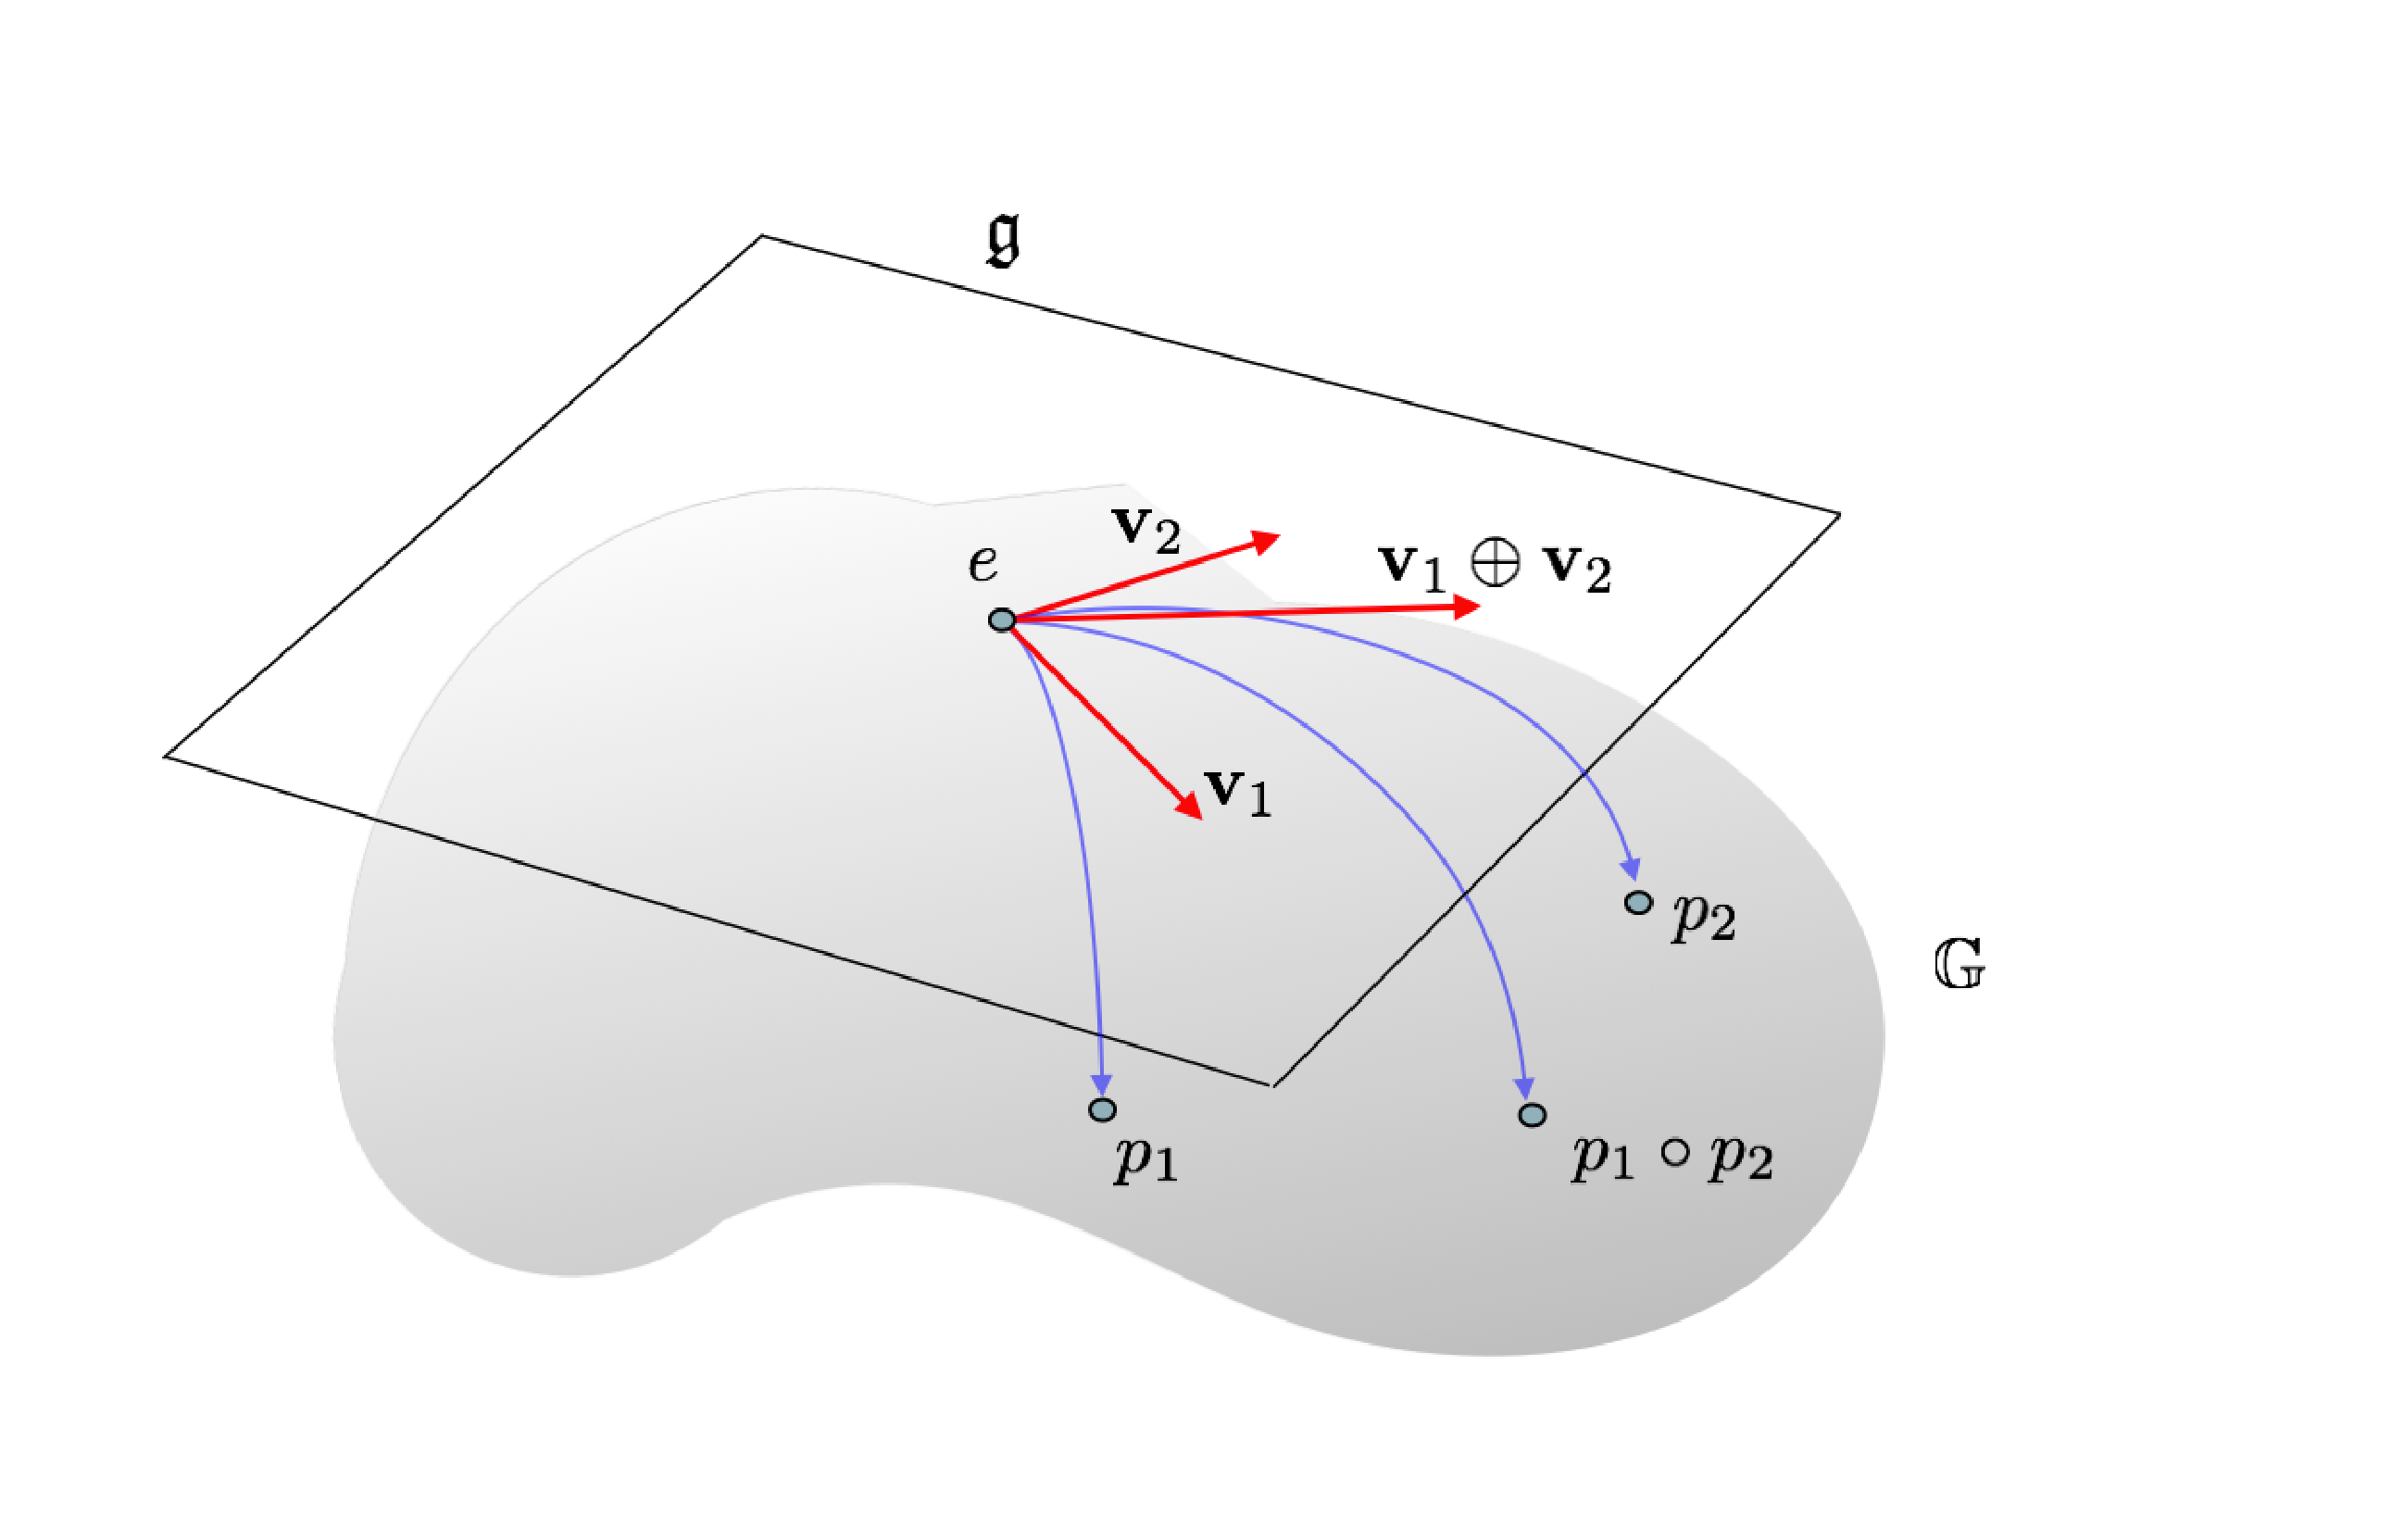
\includegraphics[scale=0.35]{figures/log_composition.pdf}
	\caption{graphical visualization of the Lie log-composition $\mathbf{v}_{1}\oplus \mathbf{v}_{2}$. The gray surface represents a Lie group and its tangent plane represents its Lie algebra. }
	\label{fig:composition}
\end{figure}

% schematical overview
A schematic overview of this formula can be visualized in figure \ref{fig:composition}. The Lie group, indicated with $\mathbb{G}$, is represented by the gray surface, while the Lie algebra, indicated with $\mathfrak{g}$, is represented by the tangent plane at the identity $e$.
Starting from the two vectors $\mathbf{v}_1$ and $\mathbf{v}_2$ in $\mathfrak{g}$, their log-composition provides the vector that corresponds to the composition of the transformations that corresponds to the initial vectors. 

% 
The analytic solution to an equivalent problem of the log-composition is provided by the BCH formula (see \cite{hall2015lie} for a formal introduction in the case of matrices). It was proved in $1947$ by Dynkin \cite{dynkin1947calculation} under the hypothesis that both the Lie exponential and Lie logarithm can be expressed in power series:
\begin{align*}
BCH(\mathbf{u},\mathbf{v}) 
= 
\mathbf{u} + \mathbf{v} + \frac{1}{2}[\mathbf{u},\mathbf{v}] + \frac{1}{12}([\mathbf{u},[\mathbf{u},\mathbf{v}]]
+ [\mathbf{v},[\mathbf{v},\mathbf{u}]]) - \frac{1}{24}[\mathbf{v},[\mathbf{u},[\mathbf{u},\mathbf{v}]]] +... 
\end{align*}
It consists in an infinite series of growing nested \emph{Lie bracket} (a bilinear form defined within the Lie algebra structure, that reflects the geometrical curvature of the space of transformations - see in particular \cite{misner1973gravitation} for a geometrical perspective on this definition).

There are many issues, both theoretical and practical that prevent from the use of this formula for practical applications. The first and most obvious is that it is an infinite series which truncations does not possess any asymptotic behaviour.
In addition, even considering a large enough number of terms, the Lie bracket of two tangent vector of the Lie group of diffeomorphisms involves the computation of the Jacobian matrices: this raises some numerical problems presented in section \ref{se:jacobian_problem}.

On the theoretical side, the proof of the BCH is based on the fact that Lie logarithm and exponential have to be expressed in power series. This happen only when the Lie group and its Lie algebra are subsets of a bigger algebra where scalar product, product and composition are compatible. This happens for matrix Lie groups (see \cite{hall2015lie} for its definition), but in the case of diffeomorphisms, the matter is not free of deceptions. The section \ref{se:svf} is devoted to the research of a bigger algebra that contains both Lie group of diffeomorphisms and its Lie algebra.
 
These are all good reasons to avoid the BCH formula when it is possible. In this thesis we will present two numerical mthods for the computation of the log-composition that does not rely on the truncated BCH - called here \emph{BCH-free} methods. The first one is based on the Taylor expansion and its formulation holds in the case of matrices. The second one, is based on a geometrical construction on the differentiable manifold of the transformation that exploit the concept of parallel transport. See \cite{do1976differential} and \cite{misner1973gravitation} for an introduction on this last concept.

Results are examined on both the Lie group of diffeomorphisms, and the matrix Lie group of rigid body transformation of the plane. In this second structure is possible to evaluate the performance on a space where all the closed form are known and the ground truth are known.





% % % % % % % % % % % % % % % % % % % % % % % % % % % % % % % % % % % % % %
% % % % % % % % % % % % % % % % % % % % % % % % % % % % % % % % % % % % % %
\section{Feasible Applications of the Log-composition in Medical Imaging}\label{se:applications_log_com_in_med}
% Quali sono le applicazioni pratiche della log composition
One of the reasons why mathematics is considered a powerful tool is consequence of the fact that a concept defined to solve a particular problem can, at the same time, be used to solve other problems from totally different origin and nature - this is known as the \emph{unreasonable effectiveness of mathematics in the natural sciences} \cite{wigner1960unreasonable}. In consequence of this, the more general and abstract is the tool developed, the more is versatile it become, but at the same difficult to understand.

The log-composition has been defined in this chapter from the problem of the computation of the statistics on the group of diffeomorphisms, but its use is not limited to perform only this task.
In medical imaging there are several other situations in which its fast and accurate computation can be helpful:
\begin{enumerate}
	\item Diffeomorphic demons \cite{vercauteren2007non} and log-demons algorithm \cite{vercauteren08}. In particular in the log-demons, the update at each of the iterative step is computed in the tangent space, using an equivalent formulation of the log-composition. 
	\item Fast computation of the logarithm computation \cite{Bossa:08}. Details of this algorithm are a part of this research and are discussed in chapter \ref{ch:log_algorithm}.
	\item Calculus on diffusion tensor \cite{Arsigny:MRM:06}. The logarithmic multiplication and the logarithmic scalar multiplication here defined, provides the Lie group with a structure of vector field. The log-composition $\oplus$ here proposed provides the Lie algebra with a structure that reflects the composition of the group.  
	\item Image set classification \cite{huanglog}. As based on the log-euclidean framework, could exploit the property of having the group composition in the tangent space.
	\item Computation of the the discrete ladder for the parallel transport \cite{Lorenzi:discrete_ladders:14}. An equivalent of the log-composition is utilized for the computation of the parallel transport.
\end{enumerate}	

Before moving to the next chapter, aimed to present the numerical techniques for its computation, it is worthed to spend a couple of words about the infinite dimensional Lie group of diffeomorphism.


 % % % % % % % % % % % % % % % % % % % % % % % % % % % % % % % % % % % % %
 % SUB SECTION
 % % % % % % % % % % % % % % % % % % % % % % % % % % % % % % % % % % % % %
\section{Thesis' Outline}\label{se:thesis_outline}
%Four chapters, all alike in dignity are presented in this fair thesis: \\
\begin{enumerate}
	
	\item[{\bf Chapter \ref{ch:tools}}] The next chapter is devoted to the mathematical elements and tools involved in the numerical methods for the computation of the log-composition.
	
	\item[{\bf Chapter \ref{ch:spatial_transformations}}] In this chapter we introduce the two sets of transformations on which the numerical methods will be tested and compared: the finite dimensional group of rigid body transformation and the infinite dimensional Lie group of diffeomorphisms.

	\item[{\bf Chapter \ref{ch:log_algorithm}}] The algorithm proposed in \cite{bossa2008algorithms} for computation of the Lie logarithm uses an equivalent formulation of the log-composition in its main core. In this chapter we will see how the numerical methods developed in the previous chapter will be utilized in this context.
  
	\item[{\bf Chapter \ref{ch:results}}] This chapter is devoted to the presentation of the numerical results applied to synthetic data and clinical images. 
	
\end{enumerate}


% % % % % % % % % % % % % % % % % % % % % % % % % % % % % % % % % % % % % %
% % % % % % % % % % % % % % % % % % % % % % % % % % % % % % % % % % % % % %
\section*{A Short Remark about the Lie Group of Diffeomorphisms}

So far we have talked about the group of diffeomorphisms as a Lie group in a natural way, without underlining any particular feature of this concept. Actually, the topic of infinite dimensional Lie gorup is an open field of research whose development has not yet reached a definitive formalization.
Aimed to presenting the theoretical problem and difficutlies as well as how we deal with them in this Master Thesis, we retrace the main historical steps and some of the most significant approaches.

The first attempt to provide some handles to the group of diffeomorphisms for easy manipulation was done by Vladimir Arnold in 1966 \cite{arnold1966geometrie} (consider also the equivalent \cite{arnold1998topological}, more readable for non-French speakers). To solve differential equation in hydrodynamic, the set of diffeomorphisms $\text{\emph{Diff}}$ is considered as a Lie group possessing a Lie algebra. This assumption is not formally explained in accordance to the problem-oriented nature of this paper. 

Subsequent steps in the exploration of the set of diffeomorphisms as a Lie group, and in the attempt of finding a formalization can be found in \cite{marsden1970hamiltonian, ebin1970groups, omori1970group, michor1980manifolds, leslie1983lie}. A state of the art of  infinite dimensional Lie group in the early eighties can be found in \cite{Milnor:84:remarks}, while more recent results and applications on diffeomorphisms have been published in \cite{ovsienko1992integrals, bauer2010sobolev, schmid2010infinite,  bauer2011geodesic}.

Considering an infinite dimensional group as a differentiable manifold implies the idea of having each of its elements in local correspondence with some generalized \lq\lq infinite-dimensional Euclidean\rq\rq\phantom{z}space. Attempts to set this correspondence showed that, the transition maps are smooth over the Banach spaces. This led to the idea of Banach Manifolds. It has been shown \cite{khesin2008geometry} that the group of diffeomorphisms defined as a manifold does not belongs to the category of Banach manifold but requires an even more general space on which the transition maps are smooth: the Frechet space. Here, important theorems from analysis, as the inverse function theorem, the Frobenius theorem, or the main results from the Lie group theory in a finite dimensional settings, as Lie correspondence theorems, do not hold anymore. 

These difficulties led some researchers to approach the set of diffeomorphisms from other perspectives: 
for example, instead of treating $\text{\emph{Diff}}$ as a group equipped with differential structures, it is seen as a quotient of other well behaved groups \cite{wojtynski1994one}. In other cases, as in \cite{marsden1970hamiltonian} first and in \cite{milnor1984remarks} later, Banach spaces are substituted with more general locally convex spaces to underpin the definition of smooth manifolds (an formal introduction to the infinite dimensional linear Lie groups, group of smooth maps and group of diffeomorphisms can be found in \cite{neeb2006infinite}).

For the medical imaging purposes, it is not necessarily to consider the general theory of infinite dimensional manifolds; we can take into account only diffeomorphisms which are interesting for our practical applications, i.e. the one defined on a compact subset $\Omega$ of $\mathbb{R}^d$. Moreover, without denying the importance of fundamentals and underestimating the doors that research in infinite dimensional Lie group theory may open, we will approach diffeomorphisms in as similar way of what has been done in set theory: we will use a \emph{naive approach} to infinite dimensional Lie group. 
Here the fundamental definition of infinite dimensional Lie group is a generalization of the finite dimensional case of matrices, and it is left more to the intuition than to a robust formalization. 




